%!TEX root = ../../main.tex
%----------------------------------------------------------------------------
\chapter{Robot Cell Design}\label{chap:robot_cell_chapter}
%----------------------------------------------------------------------------
Equipped with a robot manipulator, a gripper and a conveyor belt the task of the robot cell is to sort the Lego bricks delivered by the mobile robot. These are dropped onto the conveyor belt which moves them closer to the camera and robot. Here the corresponding bricks ordered by the MES system should be picked and returned to the mobile robot. This is the task each robot cell has to fulfil, and just like in the case of the mobile platform, the process can be subdivided into smaller tasks, which we will introduce in the upcoming sections.


% Please keep sections separated in their designated folders and only reference them here using the input tag

%!TEX root = ../../../main.tex
%%---------------------------------------------------------------------------
\section{Hardware}
\label{sec:rc_hardware}
%%---------------------------------------------------------------------------
The following hardware elements was provided in each robot cell:

\begin{itemize}
	\item Kuka KR6 Robot
	\item PG70 Gripper
	\item Conveyor Belt with 3 phase 240V Motor
	\item ABB (ACS150-01E) Frequency Converter
	\item ABB (PM554) Programmable Logic Controller(PLC) for conveyor control
	\item SICK (M4000) Laser safety fence
	\item HD Webcam for Lego brick detection in 2D
	\item Kuka touch screen for HMI
\end{itemize}

The set-up for involved components will be discussed in details where appropriate. 

\subsection{Modifications}
The conveyor belt required some changes to be able to handle and control the flow of Lego bricks. First a funnel, see figure \ref{fig:funnel}, was added as a tip-off location for the mobile robot.

  	\begin{figure}[H]
        \centering
        \begin{subfigure}{0.48\textwidth}
			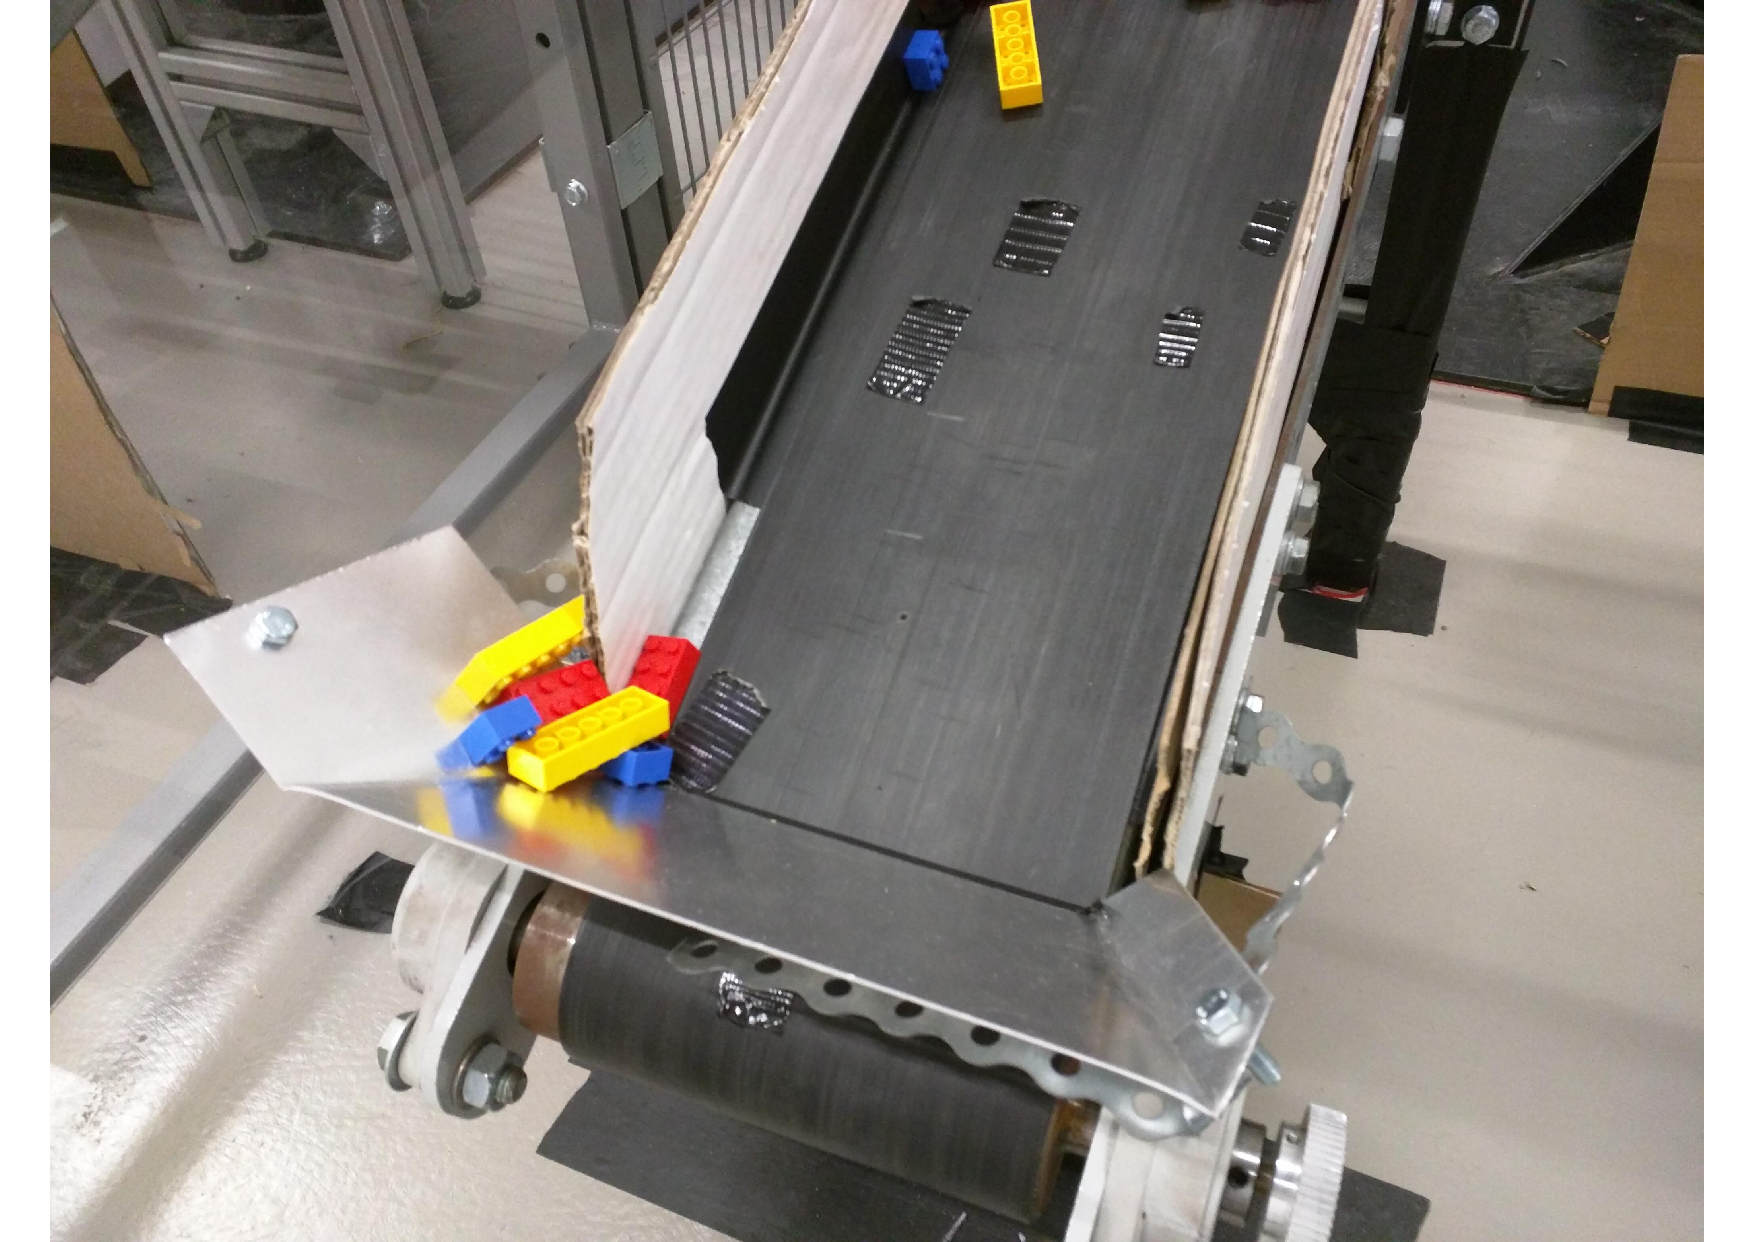
\includegraphics[width=1\textwidth]{funnel_rc}
			\caption{Funnel at delivery point for the mobile robot}
			\label{fig:funnel}
        \end{subfigure}
        \hspace{10pt}
        \begin{subfigure}{0.48\textwidth}
			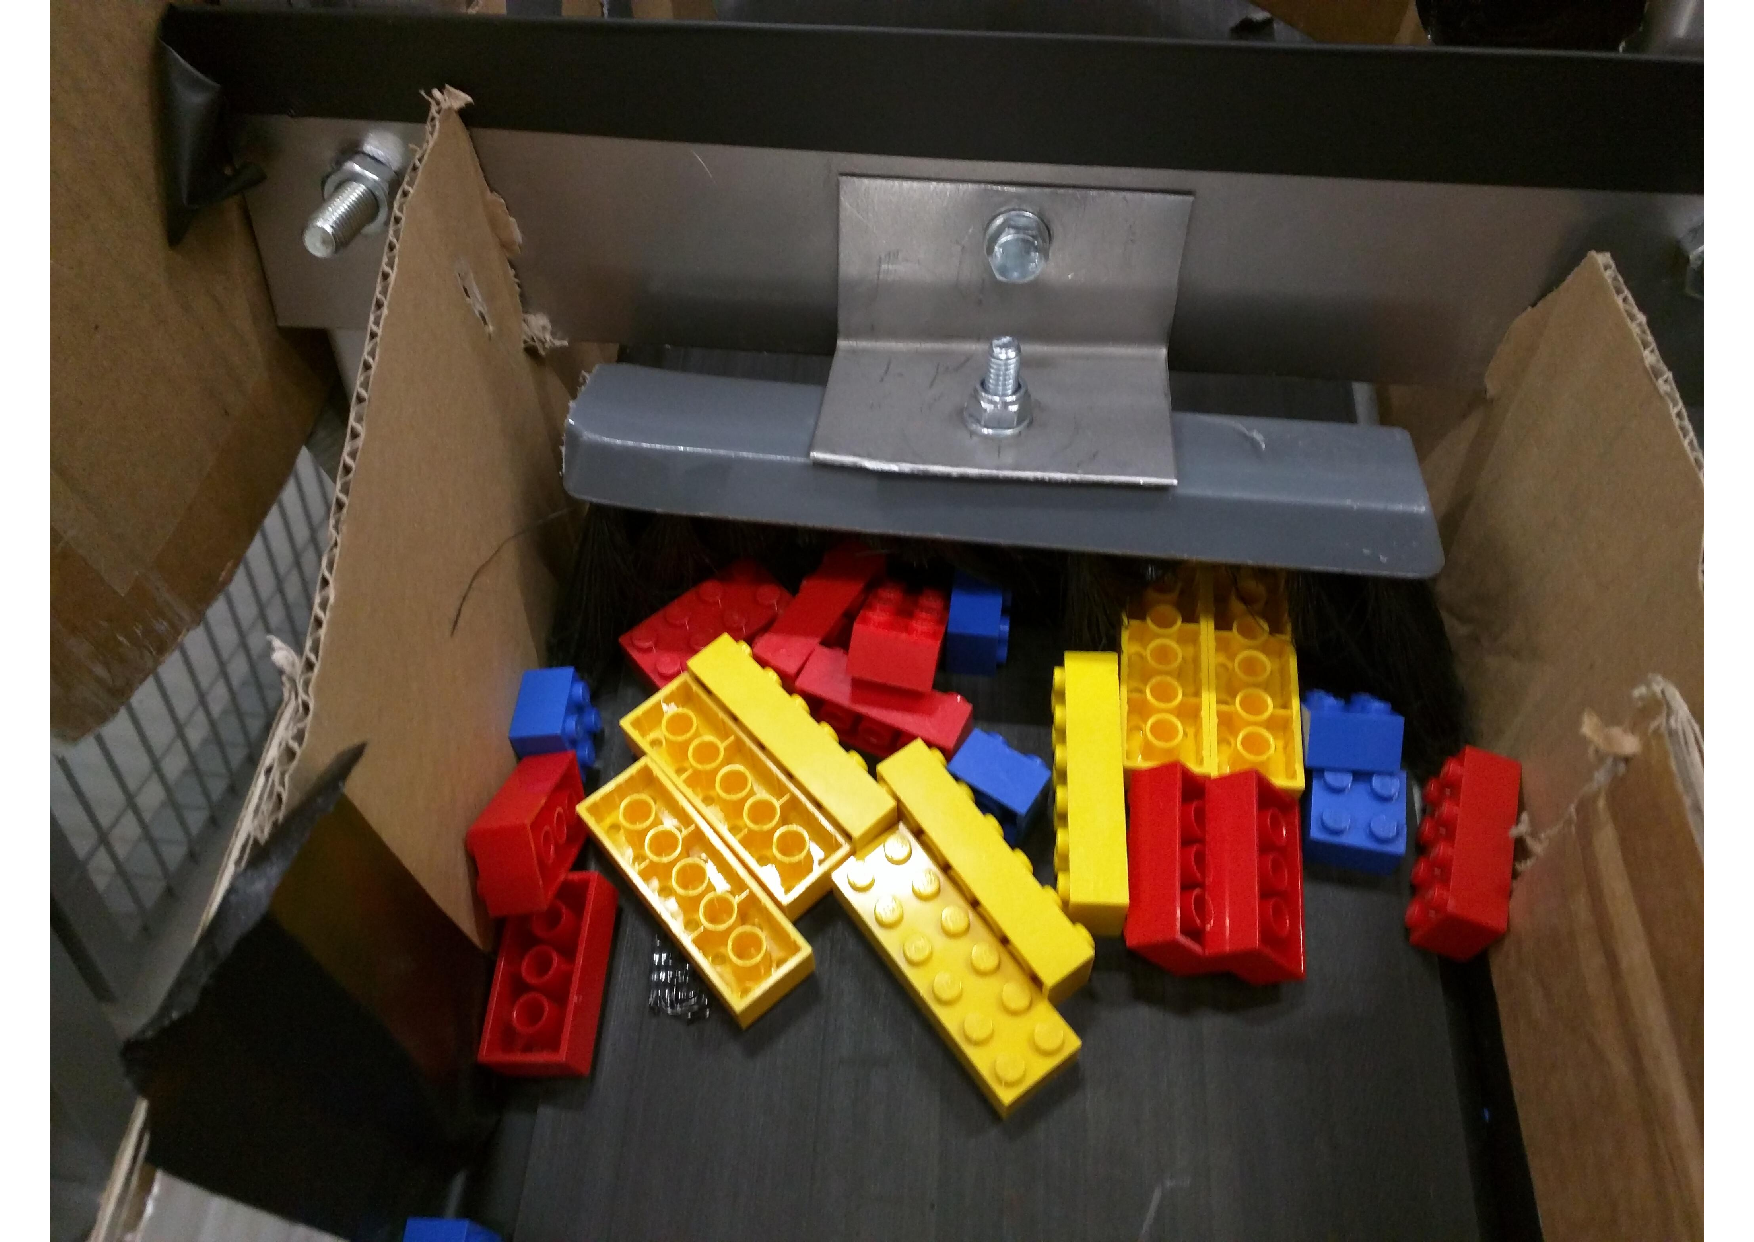
\includegraphics[width=1\textwidth]{brush_rc}
			\caption{Brush system to de-cluster the bricks}
			\label{fig:brush}
    \end{subfigure}
    \caption{Example of conveyor modifications}
    \end{figure}

Secondly, to avoid clustering and multiple layers of bricks a passive system consisting of a brush and cardboard was invented as shown in figure \ref{fig:brush}.

To provide the necessary friction to go through the system, duct tape was added at random places to the conveyor belt. See figure \ref{fig:duct_tape}.

  	\begin{figure}[H]
        \centering
        \begin{subfigure}{0.48\textwidth}
			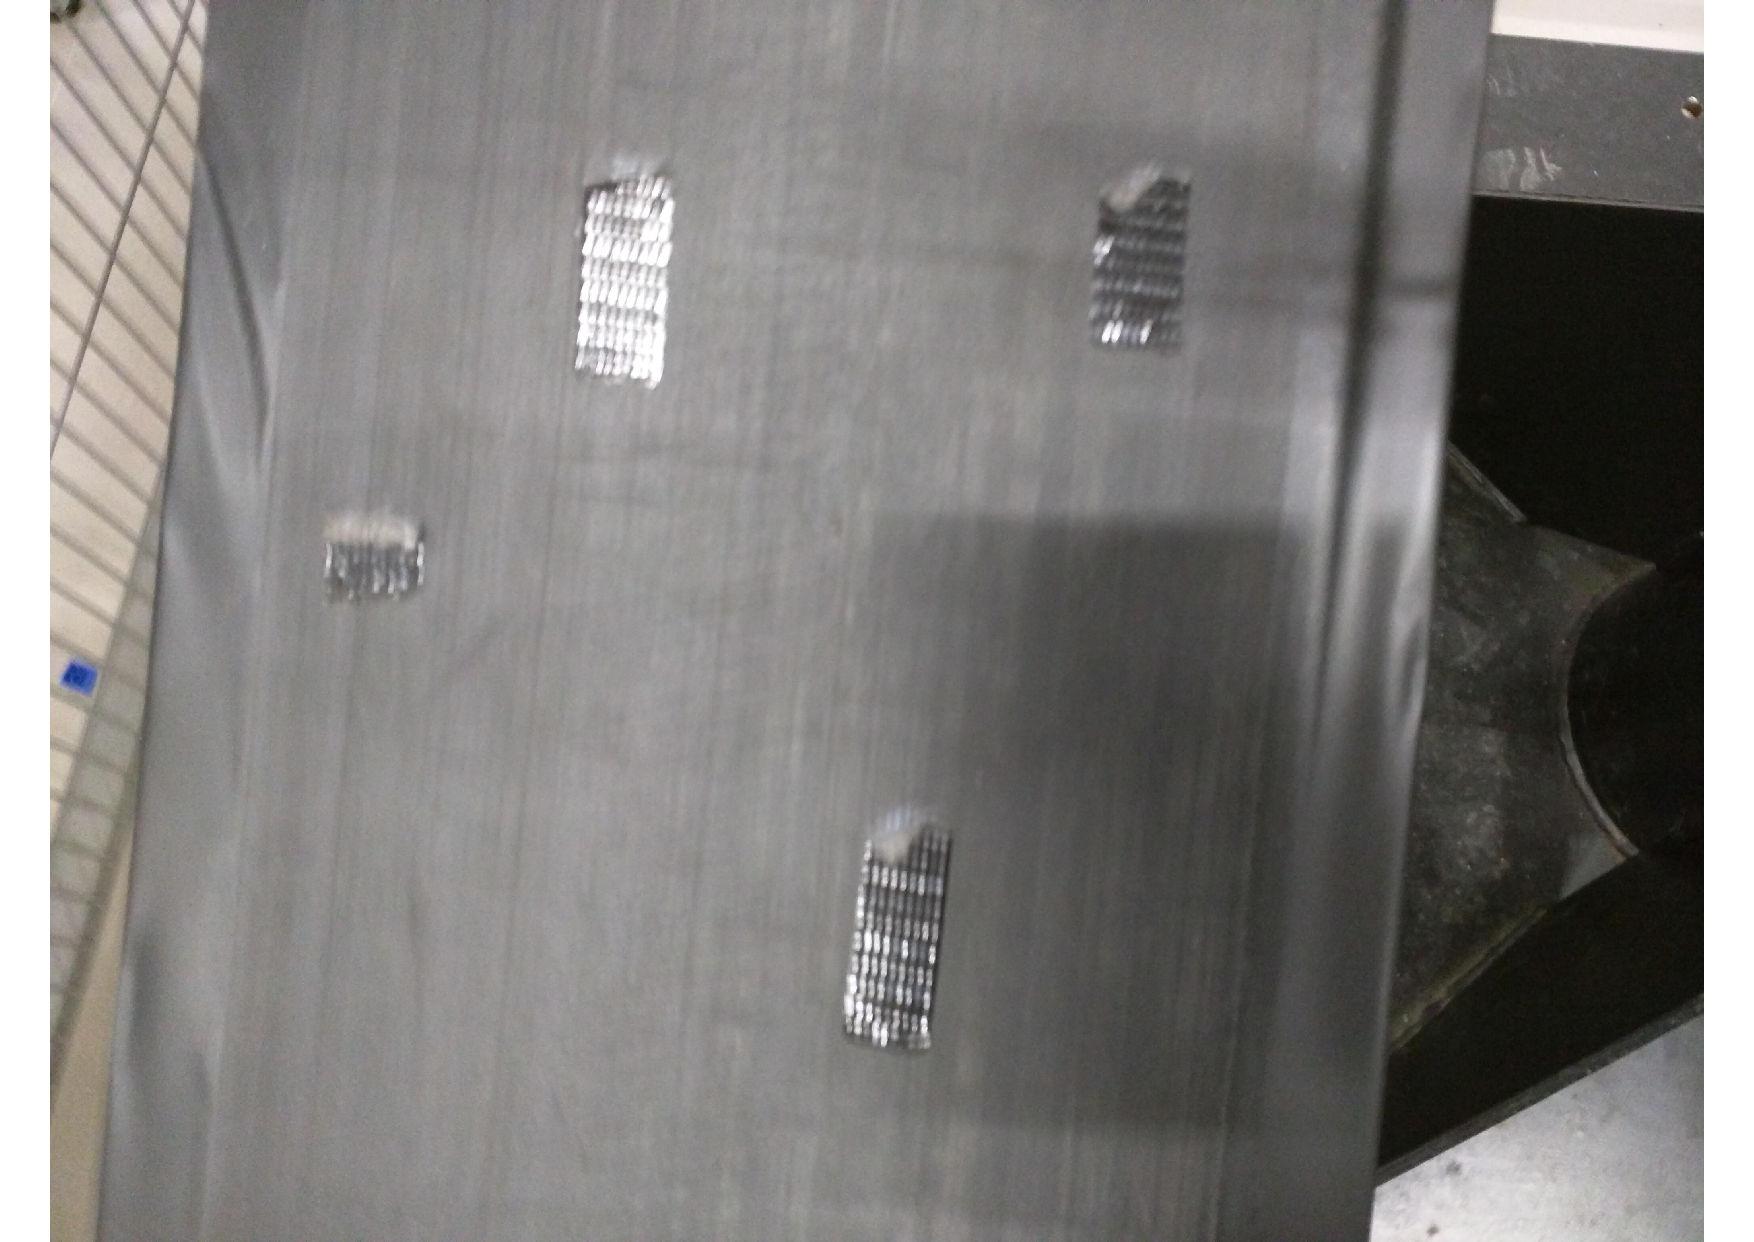
\includegraphics[width=1\textwidth]{duct_tape_rc}
			\caption{Duct tape mounted to conveyor belt}
			\label{fig:duct_tape}
        \end{subfigure}
        \hspace{10pt}
        \begin{subfigure}{0.48\textwidth}
			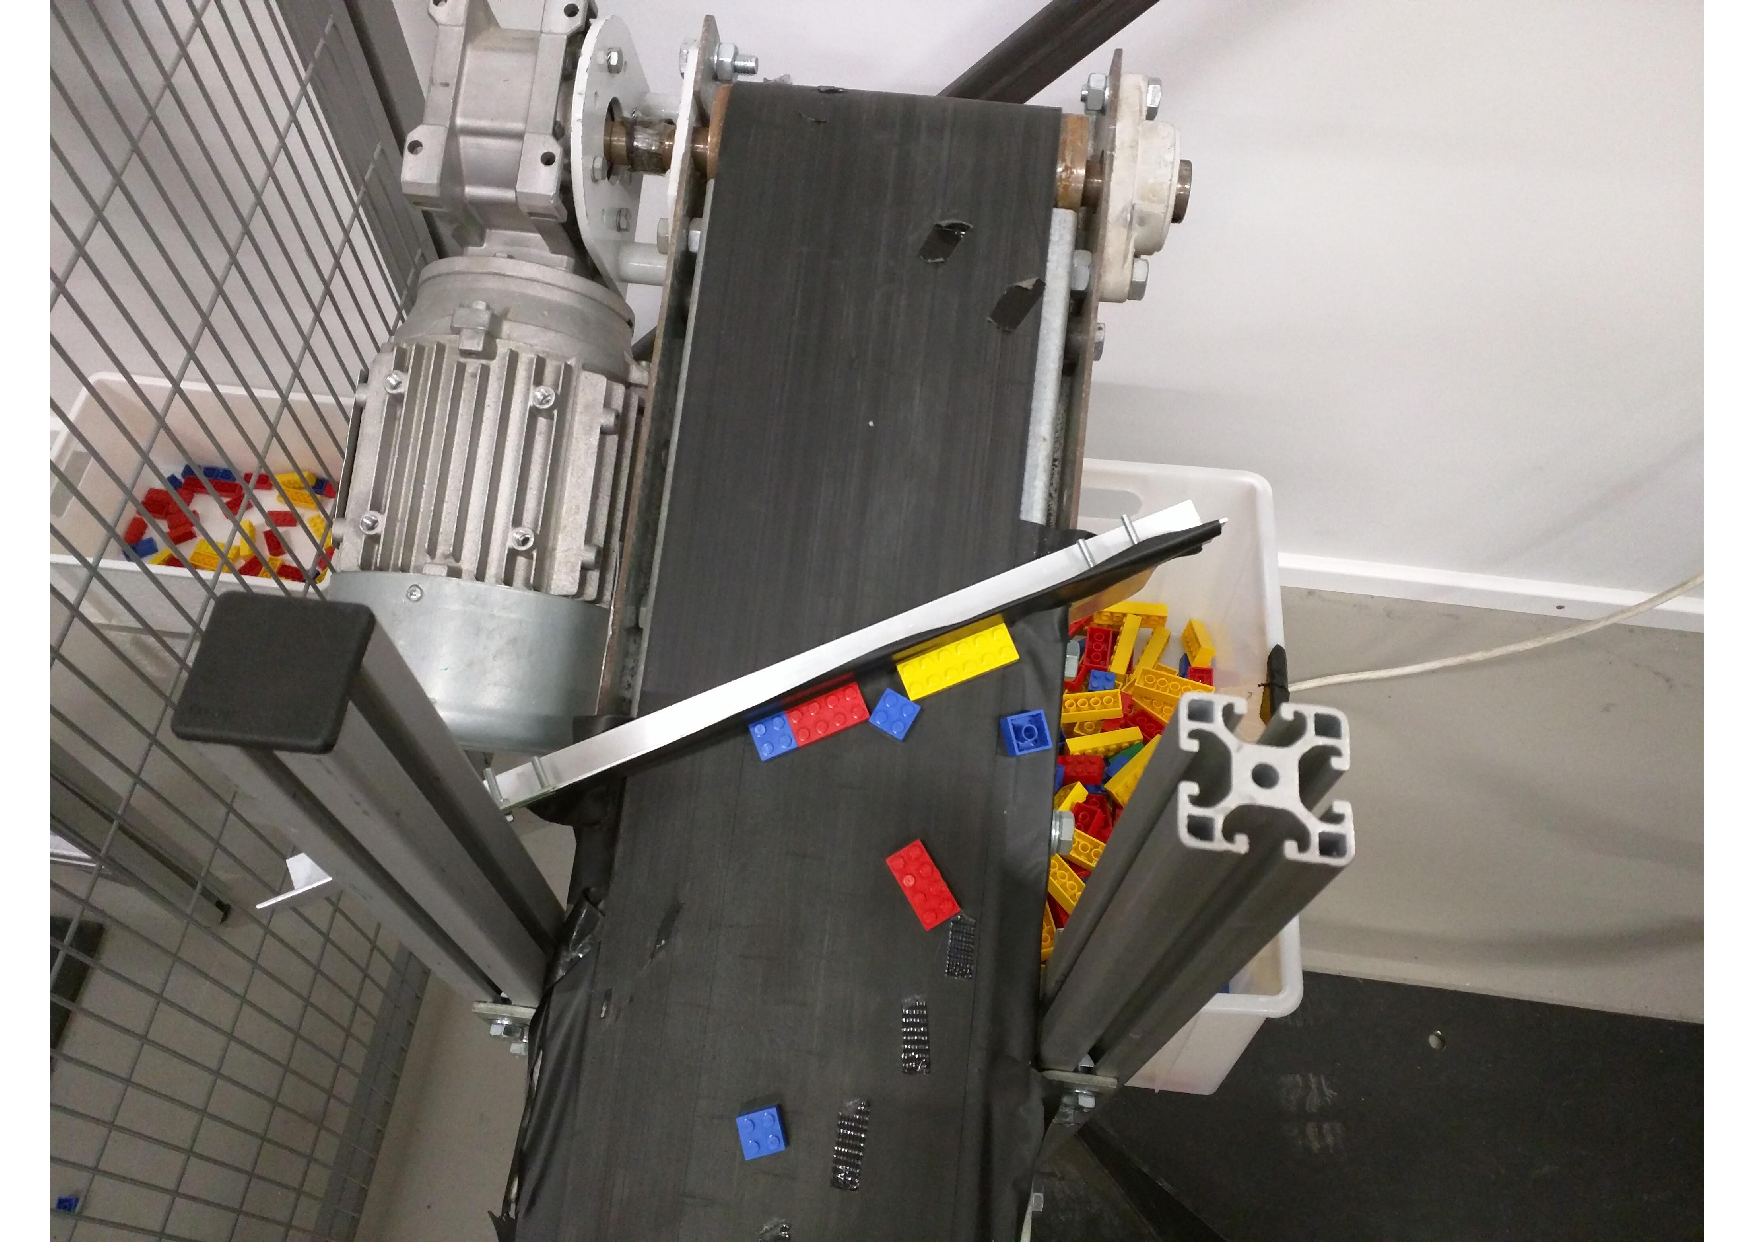
\includegraphics[width=1\textwidth]{slider_to_box}
			\caption{Slider to ensure spare bricks to fall into the box}
			\label{fig:slider}
    \end{subfigure}
    \caption{Example of conveyor modifications}
    \end{figure}

Finally, to avoid unwanted bricks on the floor, a passive slider was mounted near end of the conveyor belt. This allows the bricks to fall into a well placed box and collected at a later time. See figure \ref{fig:slider} 

%!TEX root = ../../../main.tex
%%---------------------------------------------------------------------------
\section{Camera mounting and calibration}
\label{sec:rc_camera}
%%---------------------------------------------------------------------------
The provided camera is a \textit{Logitech webcam C930e}. The camera was mounted on the robot end effector. This was done from the hypothesis that a eye-in-hand camera/robot relationship was easier to calibrate compared to a hand-to-eye system and since there is no concerns with colliding with the camera the view can be closer to the grasping area.

Camera parameters was controlled using the video4Linux api and driver. A resolution of 1280x720 with a 30 FPS was chosen. The resolution was kept high in order to have a rich details in the image and therefore making detecting bricks more stable with a cost of increased computation time due to large image sizes. 
The auto focus of the camera was disabled and the focus was tuned manually since the camera will be fixed in place relative to the bricks.
Brightness, contrast and exposure was also manually tuned in order to capture images with minimum variance. This makes it easier to apply vision algorithms.

Camera calibration was done using the camera\_calibration ROS package. Using this tool the intrinsic parameters of the camera was calculated from images of a 9x7 chequerboard held in front of the camera in 73 different positions. Rectification of the image was then performed using the image\_proc ROS package.

%!TEX root = ../../../main.tex
%%---------------------------------------------------------------------------
\section{Work-cell modelling and calibration}
\label{sec:workcell}
%%---------------------------------------------------------------------------
..

%!TEX root = ../../../main.tex
%%---------------------------------------------------------------------------
\section{Flow control overview}
\label{sec:rc_flow_control}
%%---------------------------------------------------------------------------
	\begin{figure}[H]
		\centering
	    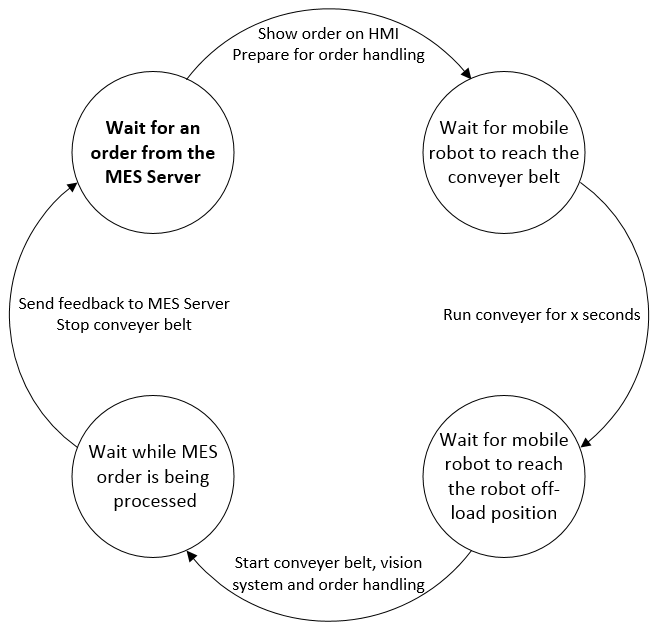
\includegraphics[width=0.75\textwidth]{rc_main_state_diagram}
	    \caption{State diagram of the robot cell}
		\label{fig:rc_main_state}
	\end{figure}
	
	\begin{figure}[H]
		\centering
	    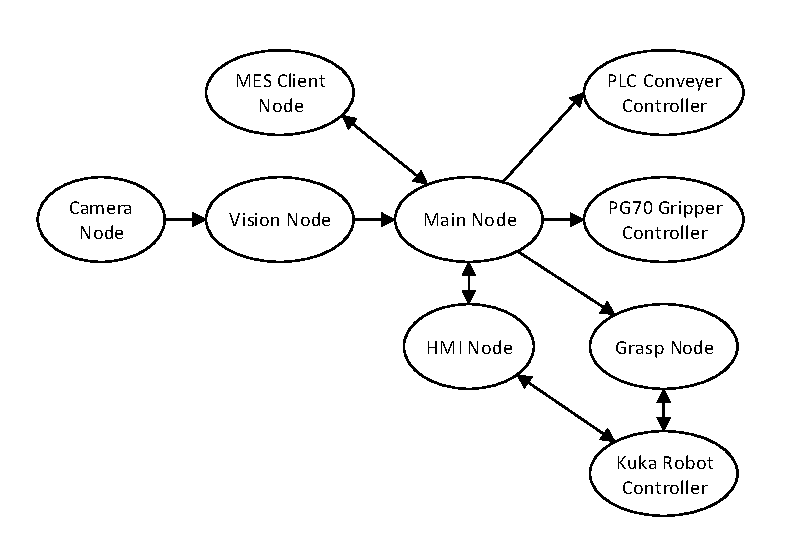
\includegraphics[width=0.8\textwidth]{rc_nodes}
	    \caption{ROS Node structure}
		\label{fig:rc_nodes}
	\end{figure}
	
%!TEX root = ../../../main.tex
%%---------------------------------------------------------------------------
\section{Kuka Robot Controller}
\label{sec:rc_kuka}
%%---------------------------------------------------------------------------
A Kuka ROS node is provided for controlling the robot arm in the robot cell. This makes it possible to communicate and exchange information such as if it is currently moving and what the configuration is. The robot can be moved in configuration space with a given speed and acceleration. \\

ROS services is provided for the above functions and acts as the interface between the Kuka actions and the main application.\\

Some issues were experienced with the Kuka setup when RSI packages was lost due to excess traffic in the switch used to connect the devices. When this occurred the robot controller stopped and the robot could not be moved before a manual reconnection. This situation could be handled by switching the state of the system to \textit{idle}, reconnecting the robot and switching back to \textit{auto}-mode. The system would then continue from the stopping point.

%!TEX root = ../../../main.tex
%%---------------------------------------------------------------------------
\section{Conveyor Belt Controller} 
\label{sec:conveyor_belt_sec}
%%---------------------------------------------------------------------------
The conveyor belt is driven by an AC motor and requires a frequency generator in order to move. The provided frequency generator can either be manually controlled or by a $24V$ digital interface. The interface between the controlling computer and the frequency generator is a PLC. A PLC is an industrial \textit{computer} with $24V$ IO interface and is logic driven. This can be programmed in different ways such as Ladder Diagrams, Structured Text and Function Block Diagrams.\\ 

The PLC in this project is programmed in Structured Text and is simply set up to respond to some serial commands. This makes it possible to start, stop and change the direction of the conveyor belt from an external serial connection.
%!TEX root = ../../../main.tex
%%---------------------------------------------------------------------------
\section{Safety} 
\label{sec:rc_safety}
%%---------------------------------------------------------------------------
The safety in the robot cell consists of a laser beam from Sick mounted in the entrance of the cell. The safety signal is directly connected the Kuka Controller unit and the robot is thus reacting immediately without requiring user interacting. This leaves the conveyor belt, gripper and the Lego sorting system aside. \\

The safety signal can be fetched through the Kuka RSI interface which is provided in ROS format. This allows the system to detect when the safety signal is changing and react upon it. This reaction consists of stopping all actions hereby all physical movements and switching state from \textit{running} to \textit{idle}. The order won't be cleared as such, making it possible to continue when the cell is safe again. \\



%!TEX root = ../../../main.tex
%%---------------------------------------------------------------------------
\section{Vision}
\label{sec:rc_hmi_sec}
%%---------------------------------------------------------------------------
The vision node has the role of detecting Lego bricks on the conveyor belt using the camera. The detection of brick includes the color, size, position and orientation. This is information that is needed in order to determine whether the brick is needed or not and how to grasp it. 

The vision Lego detection algorithm is custom made and consists of several elements from the world of vision. Figure \ref{fig:rc_vision_steps_thor} shows the steps performed on an image in order to search for bricks. These steps are described next.\\
	
	\begin{figure}[H]
		\centering
	    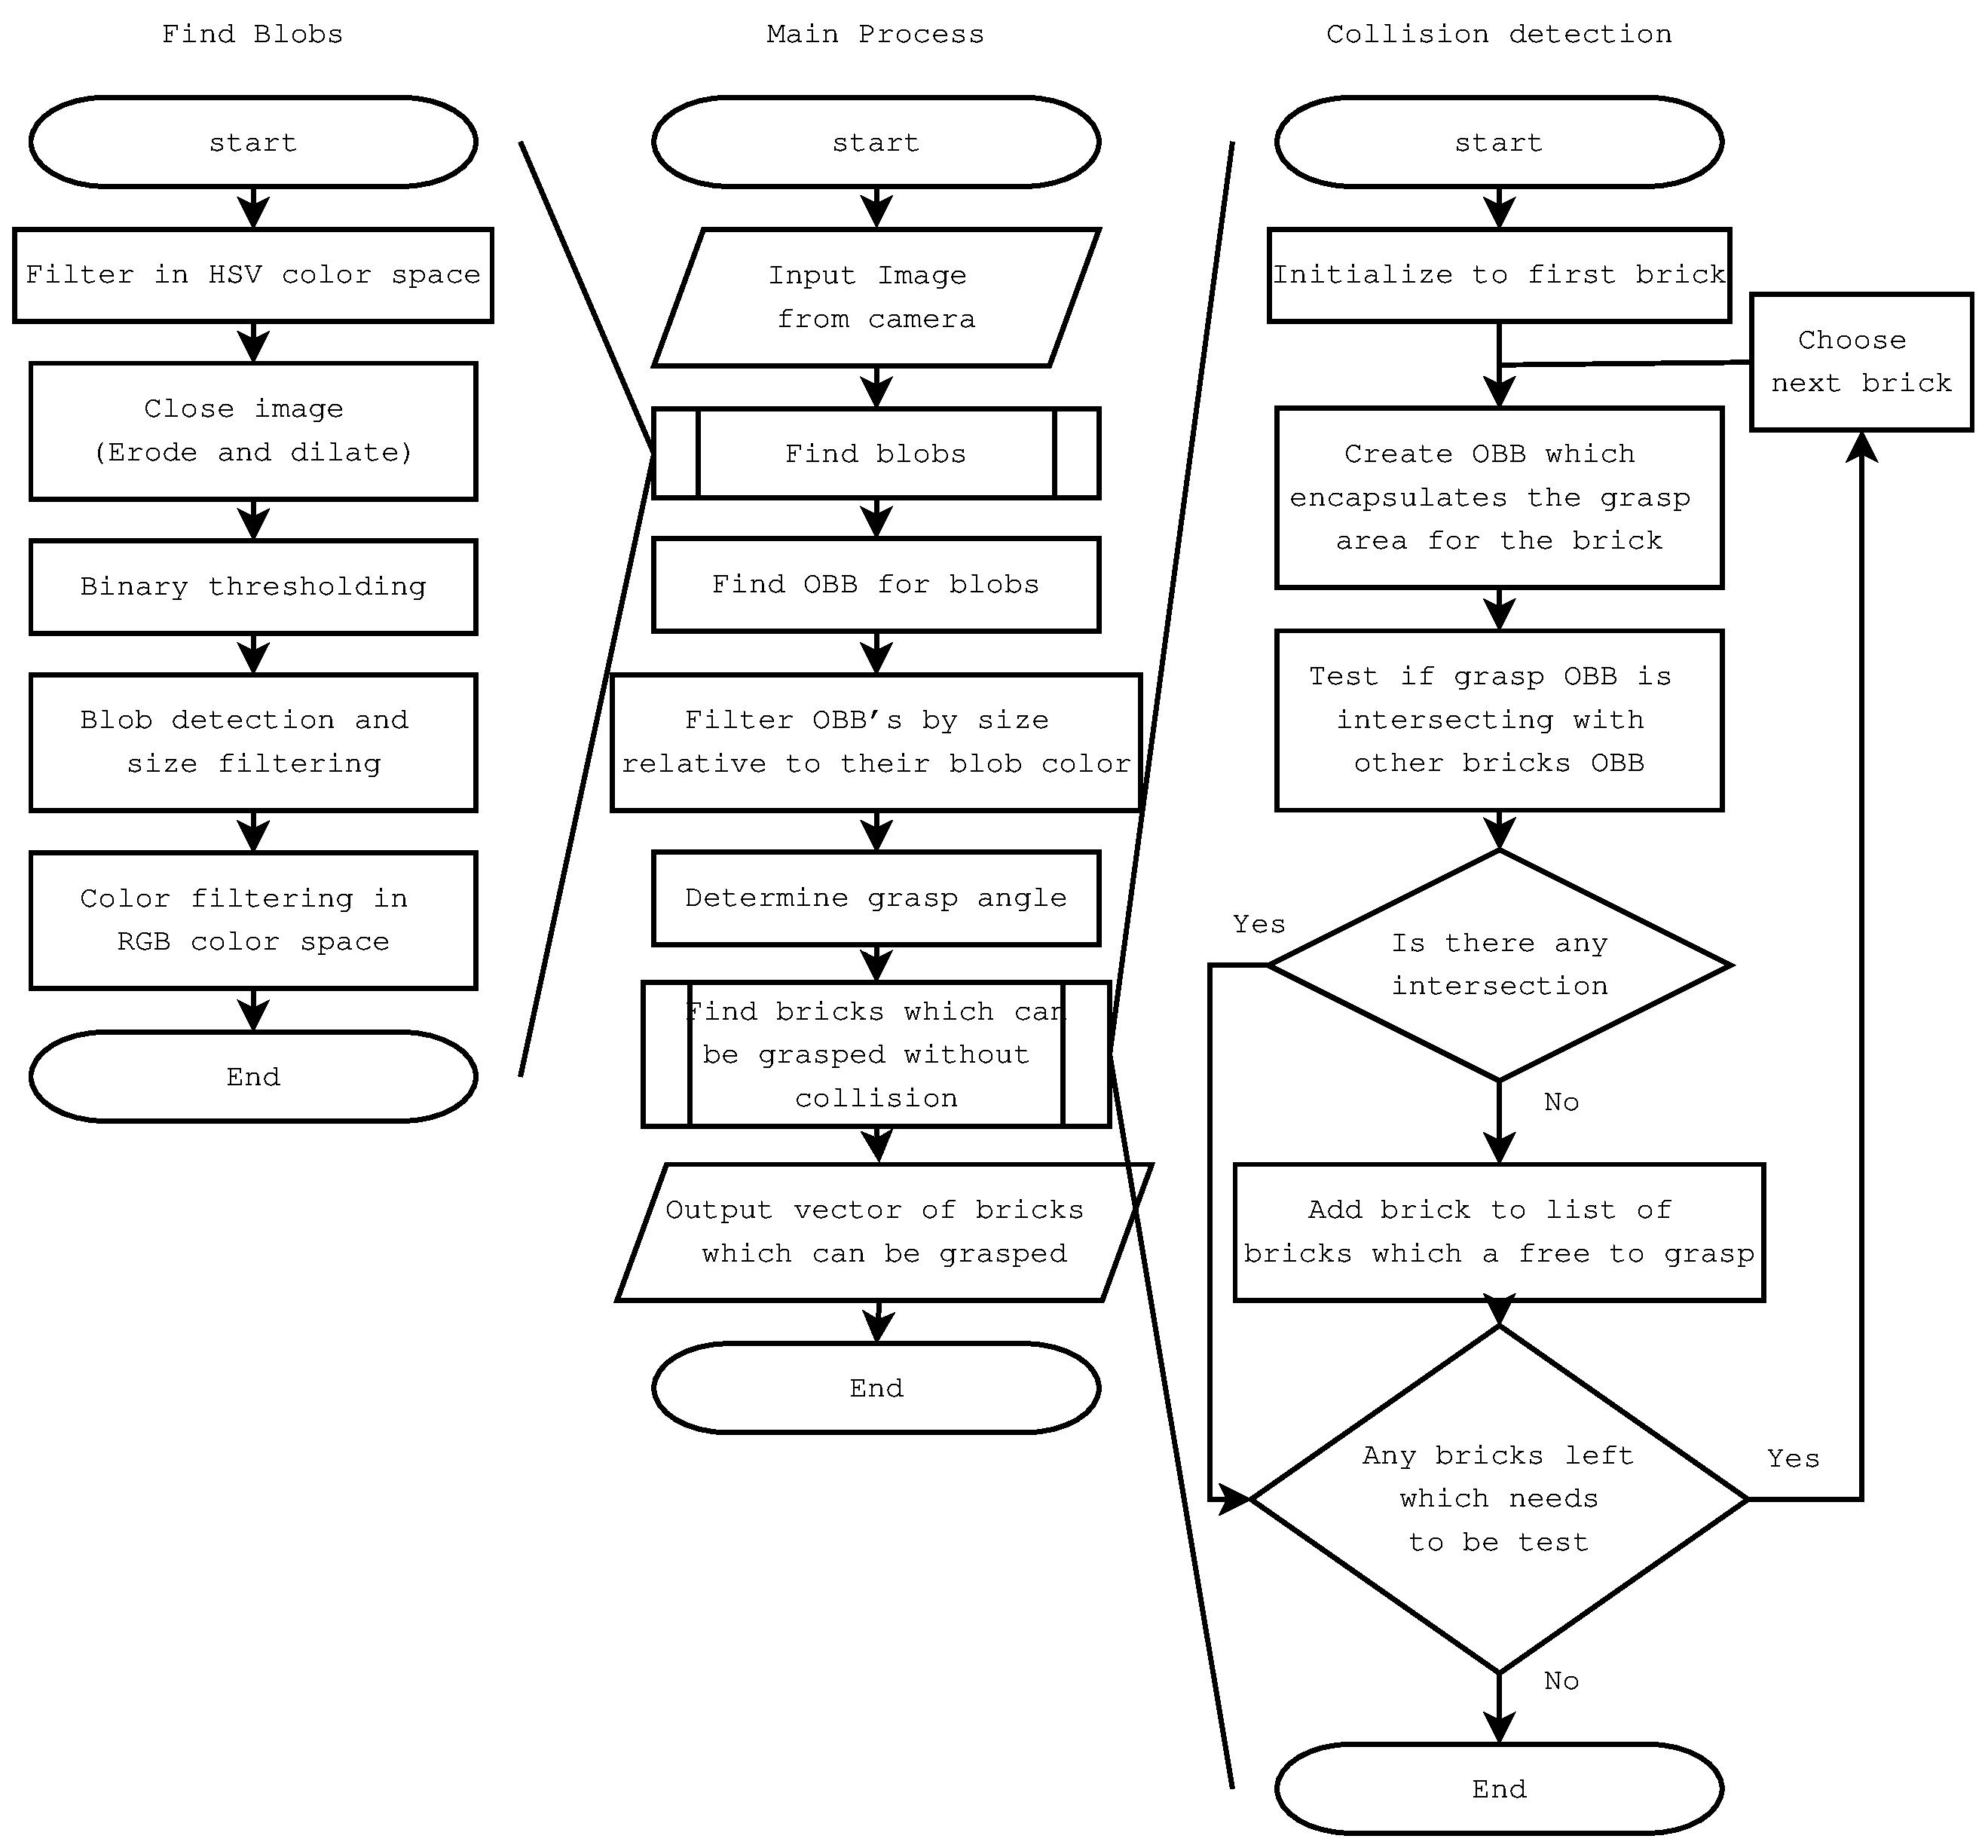
\includegraphics[width=1.0\textwidth]{rc_vision_thor.eps}
	    \caption{Steps to be performed when an image is searched for Lego bricks}
		\label{fig:rc_vision_steps_thor}
	\end{figure}
	
The vision node is able to deliver two services. One that uses a quick method to tell whether or not any bricks can be seen in the image and one that describes the image in full detail with all relevant brick information. This is used in order to save calculation time since there is no need to request the full vision algorithm if there is no bricks.

The quick method consists of only the left \textit{find blobs} part in figure \ref{fig:rc_vision_steps_thor}. This involves filtering in HSV space in order to separate the background elements from the Lego bricks. Then the image is \textit{closed} which consists of the erode and dilate process. A binary threshold is applied in order to get a binary representation of the image which is needed in blob detection. The blob detection algorithm detects the connected pixels in the image and separates them as blobs. The blobs are size filtered in order to get rid of small noisy contours. Lastly the color of the blob is determined by a custom color detection algorithm. The average RGB pixel value of all the pixels belonging the blob is calculated and the amount that the respective colors present in percentage with respect to the sum determine the correct color. Looking at the amount that the colors make up, a conclusion of the color can be made. This is robust with respect to changing light conditions and other changes to the colors. 

The next step looks into fitting oriented-bounding-boxes (OBB) to the blobs, using an OpenCV\cite{opencv} implementation. This results in the size, orientation and center position of the detected element. The size and color combination is used for further brick filtering.

The orientation of the bricks is always with respect to the y-axis of the frame and smallest side of the bricks. This makes it easy for grasp calculation and the smallest side is chosen since some Lego bricks can be too large for grasping on the longest side. 
	
	\begin{figure}[H]
		\centering
	    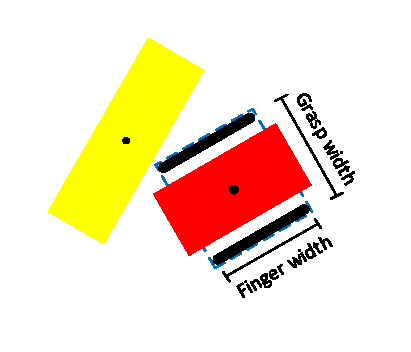
\includegraphics[width=0.5\textwidth]{rc_vision_collision.pdf}
	    \caption{Lego brick collision detection method}
		\label{fig:rc_vision_collision}
	\end{figure}
	
Finally collision avoidance is done by testing if any obstacles is in the grasp path for a brick. The grasp path for a brick is the area the two fingers of the end effector travels when trying to grasp the brick. Figure \ref{fig:rc_vision_collision} shows a example where the two bold black lines illustrates the end effector fingers. The area encapsulated by the stripped blue lines is the grasp path area for the grasp when trying to grasp the red brick illustrated by a red rectangle. A grasp path area is then tested against all other bricks except the brick to be grasped. Separating axis theorem\cite{Gottschalk:1996:OHS:237170.237244} is used to test if the rectangular grasp area is colliding with the rectangular brick areas defined by OBB's.

Since the positions of the bricks are found in the image and thus in pixels, it needs to be translated to the distance metric that the robot and gripper are using, namely meters. The pixel to meter conversion was archived using a simple method in which four corner points were marked on the conveyor and the distance between these was measured. The same distance was measured on the image in pixels. The different measurements was summed and the average scale found. It was assumed that if the set-up was kept static the scale would be valid for a longer period.

Figure \ref{fig:rc_vision_ex1} and \ref{fig:rc_vision_ex2} shows two results of the vision algorithm. The white box defines the area that a brick can be picked within. The contour of a detected brick is drawn with the color detected. The width of the contour if either thick or thin. Thick illustrates that the brick is pick-able thus not in collision and within the workspace. The green color marks a \textit{monster}, a brick or collection of bricks that is not detected as a valid brick. 

  	\begin{figure}[H]
        \centering
        \begin{subfigure}{0.45\textwidth}
            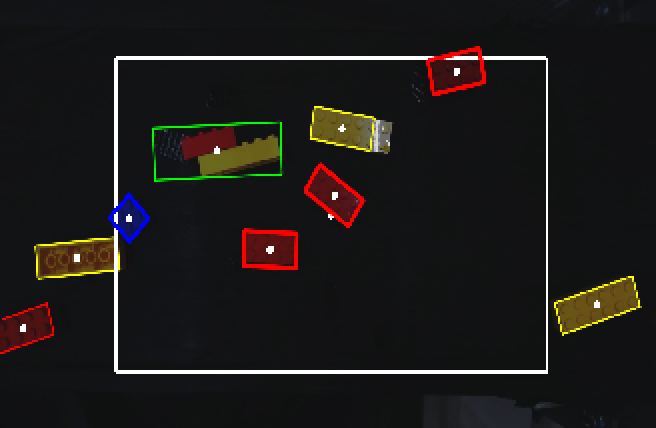
\includegraphics[width=\textwidth]{figs/rc_vision_ex1}
            \caption{}
            \label{fig:rc_vision_ex1}
        \end{subfigure}
        \hspace{10pt}
        \begin{subfigure}{0.45\textwidth}
            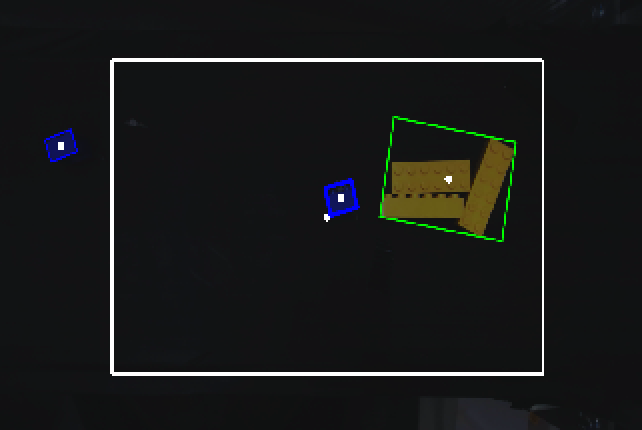
\includegraphics[width=\textwidth]{figs/rc_vision_ex2}
            \caption{Two blue bricks and a \textit{monster}}
            \label{fig:rc_vision_ex2}
    \end{subfigure}
    \caption{Example of vision output}
    \end{figure}
%!TEX root = ../../../main.tex
%%---------------------------------------------------------------------------
\section{Robot motion and grasping}
\label{sec:rc_grasp}
%%---------------------------------------------------------------------------
When a brick is detected and is in agreement with the order it needs to be picked and moved from the conveyor belt to the tipper of the mobile robot. This requires a number of robot and gripper actions. 

Figure \ref{fig:rc_grasp} shows the steps taken when a brick is to be picked. 

	\begin{figure}[H]
		\centering
	    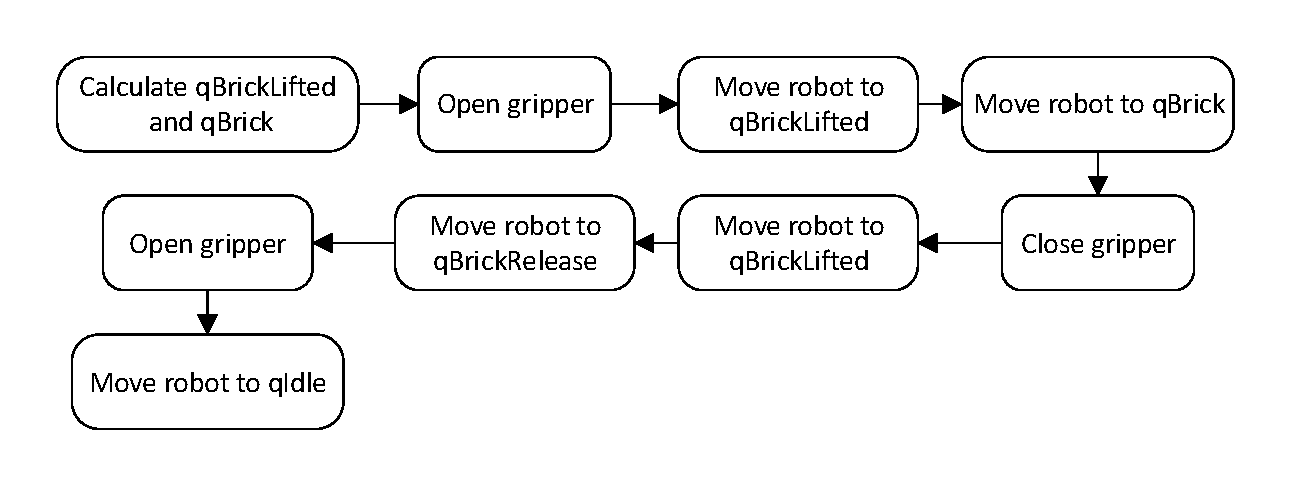
\includegraphics[width=0.95\textwidth]{rc_grasp_steps}
	    \caption{Steps performed when a Lego brick is to be picked}
		\label{fig:rc_grasp}
	\end{figure}
		
The idle position of the robot is with the z-axis of the camera frame aligned with the z-axis of the conveyor frame but with a certain distance displacement, as seen in figure \ref{fig:rc_frames}.

The calculation of \textit{qBrickLifted} and \textit{qBrick} includes inverse kinematics calculations used in order to get the position of the brick in the conveyor frame to a position in the robot frame with respect to the gripper. The configurations respectively represents the one in which the gripper and robot is aligned for grasping, but with a small offset in the z-axis and the configuration without the z-axis offset in which the gripper is in position for closing.  

No path planning is used in the process since the work-cell is static. The area in which bricks can be picked from is limited thus eliminating wrongly detected bricks resulting in collision. 


%!TEX root = ../../../main.tex
%%---------------------------------------------------------------------------
\section{Main Control}
\label{sec:rc_main}
%%---------------------------------------------------------------------------
The main component in the system is the one responsible for running the brick sorting application. The MES order is delivered to the main and it is responsible of performing the corresponding actions and starting the required services.

The brick sorting loop is only running when an order is present, the auto-mode is set, the security is okay and the robot is at the idle position. If that is the case the conveyor belt is started and the vision rough brick detector activated. When a brick is detected, the full algorithm is performed in order to match a brick with one requested in the order. The conveyor belt is only stopped if this is the case. This makes the brick sorting quite fast since a stop in the flow only occurs when a brick is to be picked. 

A security stop will at any time result in a change to idle mode and a stop of all actions. 
%!TEX root = ../../../main.tex
%%---------------------------------------------------------------------------
\section{Human Machine Interface}
\label{sec:rc_hmi}
%%---------------------------------------------------------------------------
A separate Human Machine Interface (HMI) is developed for controlling the robot cell. This allows the user to control relevant parameters from an intuitive GUI. 

The HMI is implemented as a plugin to RobWorkStudio. This allows the HMI to act alongside the visual representation of the work-cell allowing a real-time simulation of the actions.

Figure \ref{fig:rc_hmi} shows the HMI plugin. All system elements are using the log for error and information messages. The user is able to manually control the robot, conveyor and gripper. Some camera settings can be directly controlled from the HMI and the video feed shows a direct view of either the raw or vision applied image. 

	\begin{figure}[H]
		\centering
	    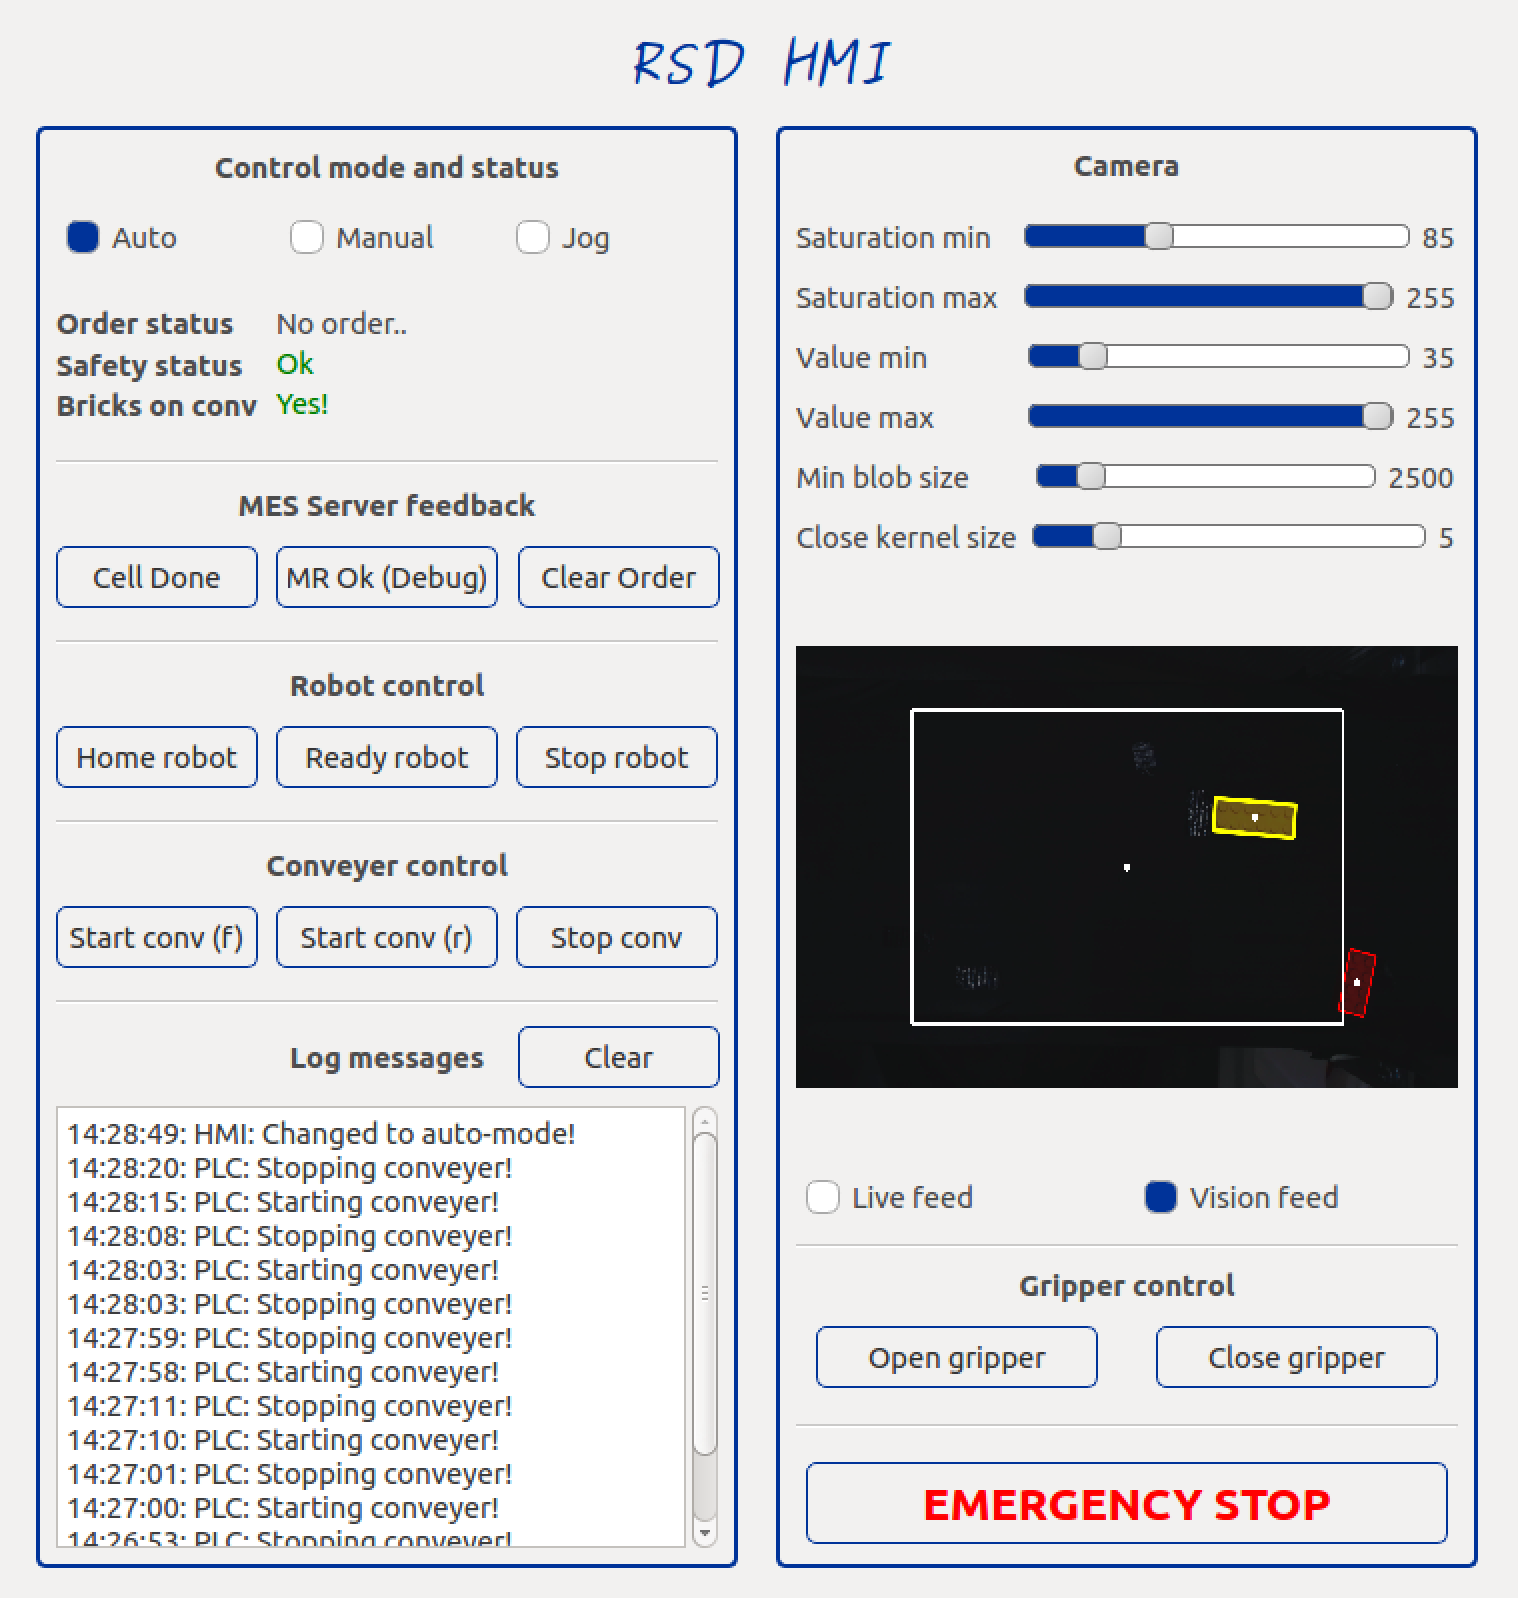
\includegraphics[width=0.9\textwidth]{rc_hmi}
	    \caption{HMI}
		\label{fig:rc_hmi}
	\end{figure}


%%% Local Variables:
%%% mode: latex
%%% TeX-master: "main"
%%% End: